\documentclass[11pt]{article}
\usepackage{url}
\usepackage{cite}
\usepackage{amsmath}
\usepackage{graphicx}
\graphicspath{{../umlet/}}

\begin{document}

\title{Notes}
\author{Ernest Kirstein}
\maketitle

\section*{Recursive Descent Parsing}

The core rules for my parser are built off of Dr. Lewis's notes \cite{lewis}.
A grammar is define as an ordered collection of production rules.
My parser uses context-free grammar rules, which are comprised of a
'head' (the single-symbol left hand side of the production rule), and a 'tail'
(one or more symbols comprising the right hand side of the production rule).

These grammars may be 'compiled' using the four procedures:
factoring, substitution, removing left recursion, and removing useless
rules. Let 'decision list' define an ordered list of production rule
choices which produces a parse tree.
As each of these four procedures produces a weakly equivalent grammar,
there exists a mapping for any decision list in a compiled grammar
back into a same-terminal-producing decision list in the pre-compiled (parent) grammer.
My parser keeps track of these inverse transformation rules as performs
it's compilation procedure so that a compiled grammar's decision list can be easily
converted to the initial grammar's equavalent decision list. 

Take this simple grammar for example:
\begin{align}
S &\rightarrow A B\\
A &\rightarrow a\\
A &\rightarrow S A\\
B &\rightarrow b\\
B &\rightarrow S B
\end{align}
It compiles into the weakly equivalent grammar:
\setcounter{equation}{0}
\begin{align}
Z &\rightarrow \epsilon\\
B &\rightarrow b\\
S &\rightarrow a B S'\\
S' &\rightarrow \epsilon\\
A &\rightarrow a Z\\
B &\rightarrow a B S' B\\
S' &\rightarrow a Z B S'\\
Z &\rightarrow b S' A\\
Z &\rightarrow a B S' B S' A
\end{align}

So when the terminal stream "aabb" is parsed in the compiled
grammar to the decision list $[3, 6, 2, 4, 2, 4]$ it can be transformed
into the parent-grammar-equivalent decision list: $[1, 2, 5, 1, 2, 4, 4]$.

\begin{figure}[p]
    \centering
    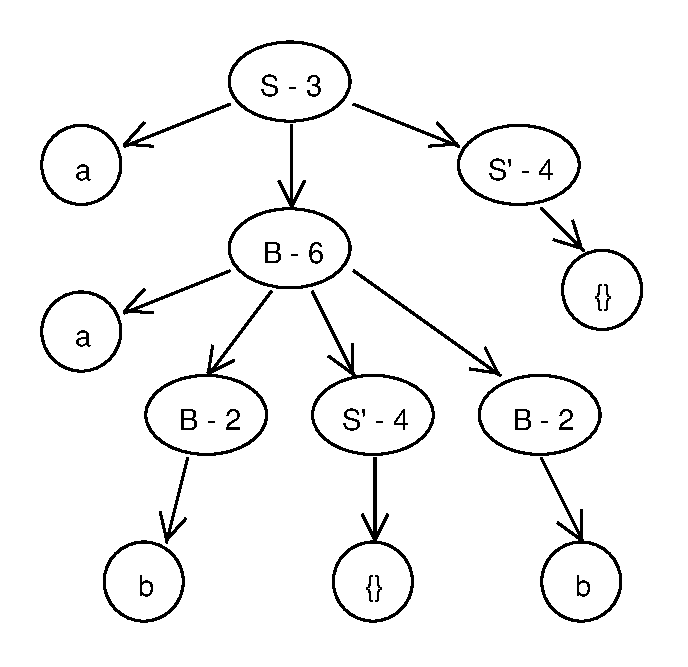
\includegraphics[width=0.8\textwidth,natwidth=458,natheight=444]{compiled_ex.pdf}
    \caption{Compiled Grammar Parse Tree}
    \label{fig:compiled_ex}
\end{figure}
\begin{figure}[p]
    \centering
    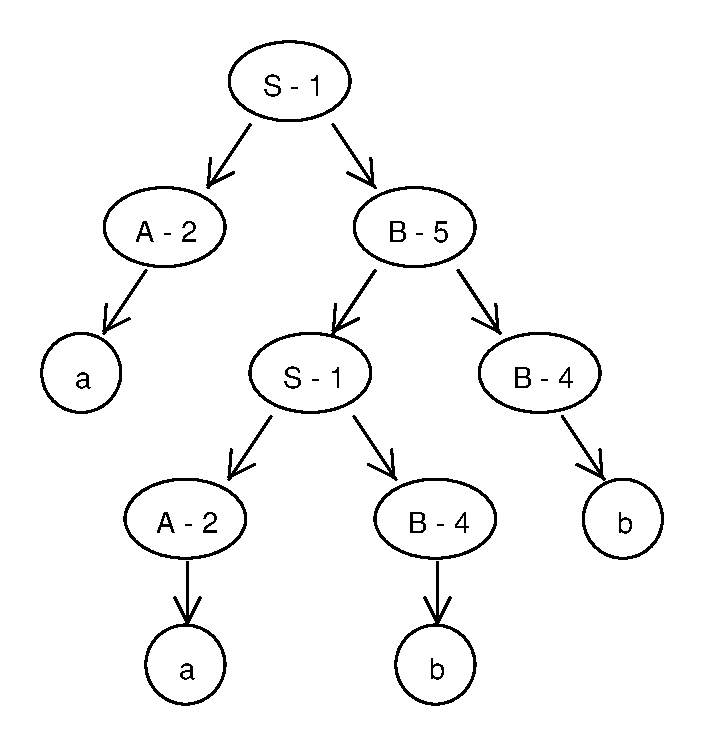
\includegraphics[width=0.8\textwidth,natwidth=472,natheight=500]{decompiled_ex.pdf}
    \caption{Parent Grammar Parse Tree}
    \label{fig:decompiled_ex}
\end{figure}

\bibliography{notes}{}
\bibliographystyle{plain}
\end{document}
